\documentclass[11pt, a4paper,twocolumn]{jarticle}
\usepackage[dvipdfmx]{graphicx}
\usepackage{listings,jlisting}

\begin{document}
%=============================================================
\section{一次元走査光学系の組み立て}
\subsection{目的}
今回の実験では走査状態での光信号の測定を行うための光学系を作成することが目的である.

\subsection{手順}
図\ref{fig:7}のように光学系を構成した.
ステッピングモーター以外の構成は前回の定常状態での光信号の取得での光学系と同じものを使用した.
半導体レーザーからコリメートされた光をステッピングモーターについている反射鏡に入射させることでモーターの制御で入力物体をx軸方向に走査して光信号を検出できるようにした.
なお,この実験では光学系を作成するのみなので結果,考察を省く.


\begin{figure}[ht]
 \begin{center}
  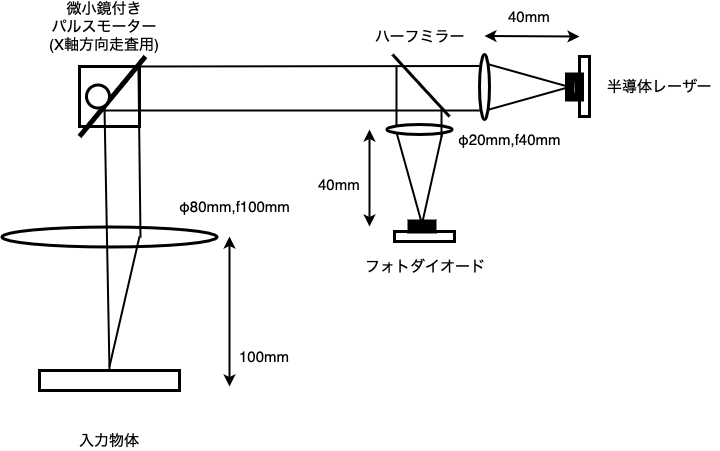
\includegraphics[width=0.8\linewidth]{fig7.png}
 \end{center}
 \caption{一次元走査光学系}
 \label{fig:7}
\end{figure}


%=============================================================
\newpage
\end{document}
